\chapter{Overview}
The wannier code should be able to operate in three modes

(1) Read in the overlaps and projections from file as computed 
inside an ab-initio code. We expect this to be the most common route to using the Wannier code.


(2) As a set of library routines to be called from within an ab-initio code. 
The ab-initio code passes the overlaps and projections to the wannier library routines
and in return gets the unitary transformation corresponding to maximally localised wannier functions.
This route should be used if the Wannier functions are needed within the ab-initio code, for example
in post-LDA methods such as LDA+U or SIC.


(3) Read in the
wavefunctions in real space from a planewave code using norm-conserving
pseudopotentials and computer the necessary overlaps and projections.
This option is present for legacy reasons and also to provide a ''quick and dirty'' way to
interface with new planewave codes.
                                                                                                                         


\begin{figure}
\begin{center}
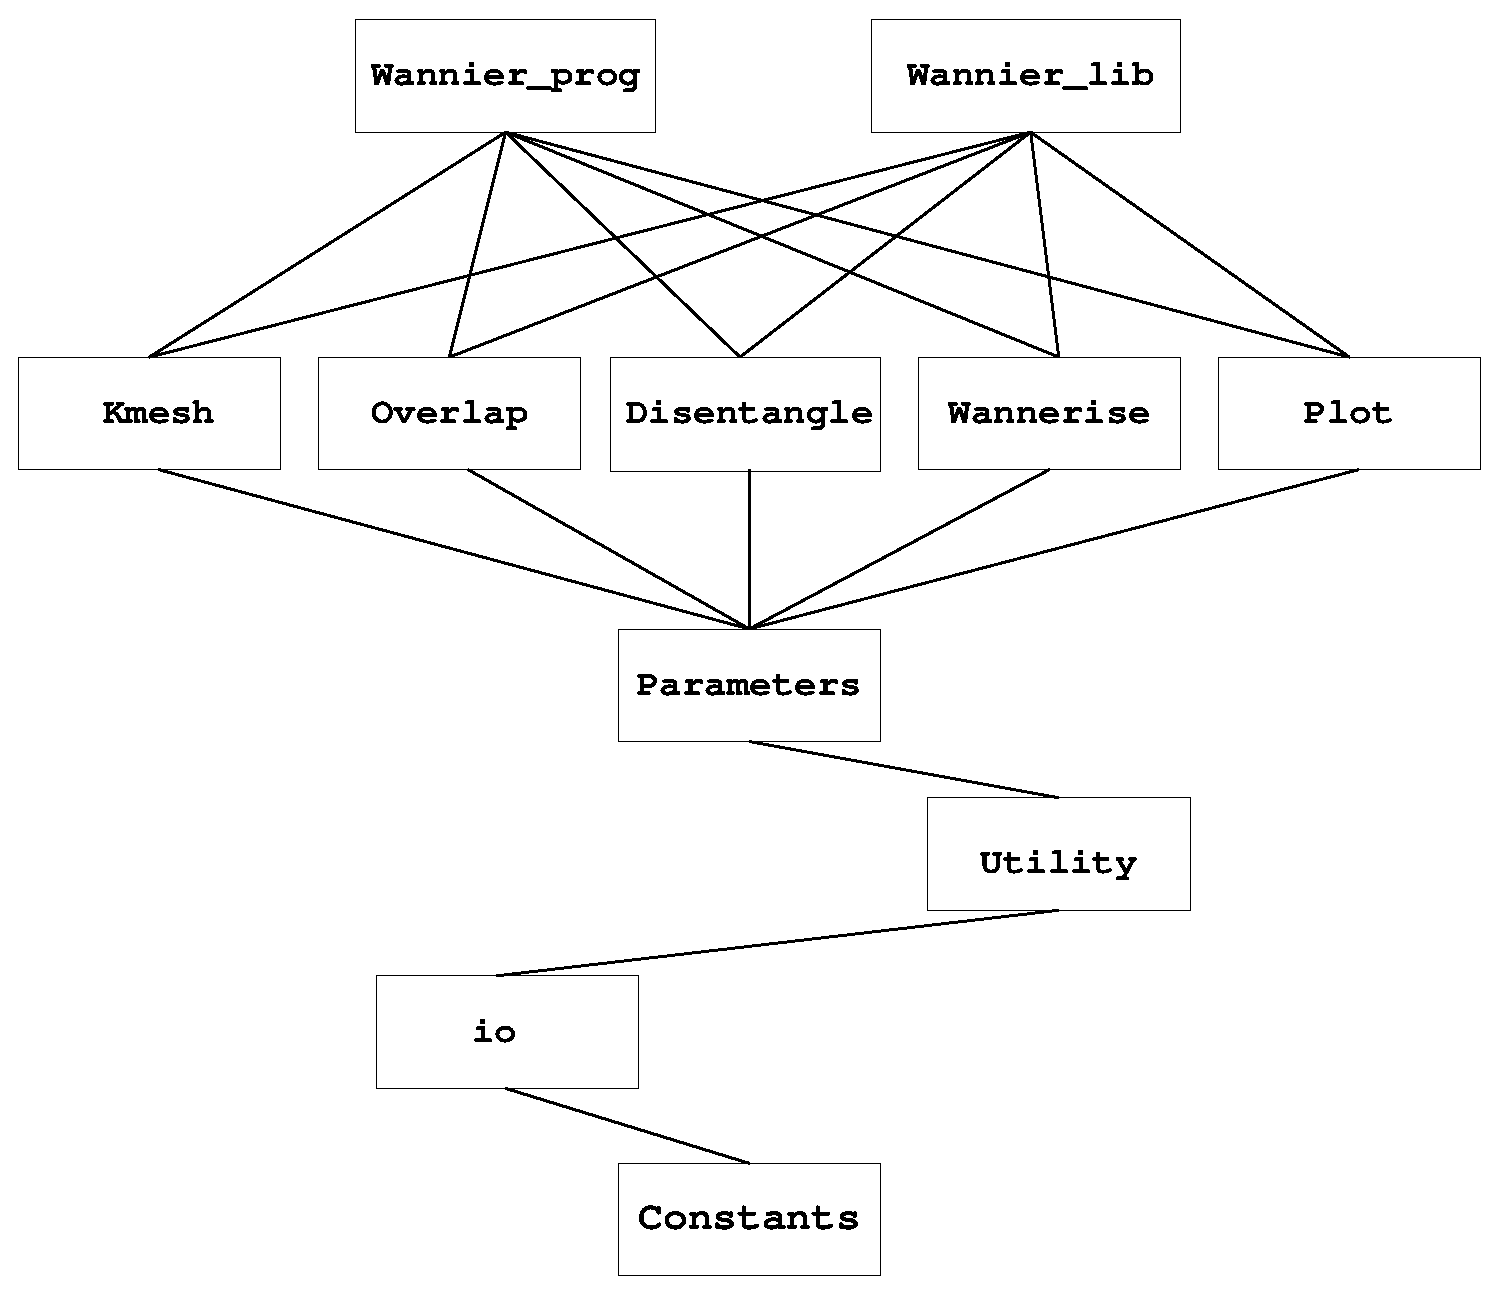
\includegraphics[width=6in]{overview.eps}
\caption{Schematic overview of the module structure of the wannier code. Modules may only use data
and subroutines from lower modules.}
\label{structure}
\end{center}
\end{figure}
